% Options for packages loaded elsewhere
% Options for packages loaded elsewhere
\PassOptionsToPackage{unicode}{hyperref}
\PassOptionsToPackage{hyphens}{url}
\PassOptionsToPackage{dvipsnames,svgnames,x11names}{xcolor}
%
\documentclass[
  letterpaper,
  DIV=11,
  numbers=noendperiod]{scrartcl}
\usepackage{xcolor}
\usepackage{amsmath,amssymb}
\setcounter{secnumdepth}{-\maxdimen} % remove section numbering
\usepackage{iftex}
\ifPDFTeX
  \usepackage[T1]{fontenc}
  \usepackage[utf8]{inputenc}
  \usepackage{textcomp} % provide euro and other symbols
\else % if luatex or xetex
  \usepackage{unicode-math} % this also loads fontspec
  \defaultfontfeatures{Scale=MatchLowercase}
  \defaultfontfeatures[\rmfamily]{Ligatures=TeX,Scale=1}
\fi
\usepackage{lmodern}
\ifPDFTeX\else
  % xetex/luatex font selection
\fi
% Use upquote if available, for straight quotes in verbatim environments
\IfFileExists{upquote.sty}{\usepackage{upquote}}{}
\IfFileExists{microtype.sty}{% use microtype if available
  \usepackage[]{microtype}
  \UseMicrotypeSet[protrusion]{basicmath} % disable protrusion for tt fonts
}{}
\makeatletter
\@ifundefined{KOMAClassName}{% if non-KOMA class
  \IfFileExists{parskip.sty}{%
    \usepackage{parskip}
  }{% else
    \setlength{\parindent}{0pt}
    \setlength{\parskip}{6pt plus 2pt minus 1pt}}
}{% if KOMA class
  \KOMAoptions{parskip=half}}
\makeatother
% Make \paragraph and \subparagraph free-standing
\makeatletter
\ifx\paragraph\undefined\else
  \let\oldparagraph\paragraph
  \renewcommand{\paragraph}{
    \@ifstar
      \xxxParagraphStar
      \xxxParagraphNoStar
  }
  \newcommand{\xxxParagraphStar}[1]{\oldparagraph*{#1}\mbox{}}
  \newcommand{\xxxParagraphNoStar}[1]{\oldparagraph{#1}\mbox{}}
\fi
\ifx\subparagraph\undefined\else
  \let\oldsubparagraph\subparagraph
  \renewcommand{\subparagraph}{
    \@ifstar
      \xxxSubParagraphStar
      \xxxSubParagraphNoStar
  }
  \newcommand{\xxxSubParagraphStar}[1]{\oldsubparagraph*{#1}\mbox{}}
  \newcommand{\xxxSubParagraphNoStar}[1]{\oldsubparagraph{#1}\mbox{}}
\fi
\makeatother


\usepackage{longtable,booktabs,array}
\usepackage{calc} % for calculating minipage widths
% Correct order of tables after \paragraph or \subparagraph
\usepackage{etoolbox}
\makeatletter
\patchcmd\longtable{\par}{\if@noskipsec\mbox{}\fi\par}{}{}
\makeatother
% Allow footnotes in longtable head/foot
\IfFileExists{footnotehyper.sty}{\usepackage{footnotehyper}}{\usepackage{footnote}}
\makesavenoteenv{longtable}
\usepackage{graphicx}
\makeatletter
\newsavebox\pandoc@box
\newcommand*\pandocbounded[1]{% scales image to fit in text height/width
  \sbox\pandoc@box{#1}%
  \Gscale@div\@tempa{\textheight}{\dimexpr\ht\pandoc@box+\dp\pandoc@box\relax}%
  \Gscale@div\@tempb{\linewidth}{\wd\pandoc@box}%
  \ifdim\@tempb\p@<\@tempa\p@\let\@tempa\@tempb\fi% select the smaller of both
  \ifdim\@tempa\p@<\p@\scalebox{\@tempa}{\usebox\pandoc@box}%
  \else\usebox{\pandoc@box}%
  \fi%
}
% Set default figure placement to htbp
\def\fps@figure{htbp}
\makeatother





\setlength{\emergencystretch}{3em} % prevent overfull lines

\providecommand{\tightlist}{%
  \setlength{\itemsep}{0pt}\setlength{\parskip}{0pt}}



 


\KOMAoption{captions}{tableheading}
\makeatletter
\@ifpackageloaded{caption}{}{\usepackage{caption}}
\AtBeginDocument{%
\ifdefined\contentsname
  \renewcommand*\contentsname{Table of contents}
\else
  \newcommand\contentsname{Table of contents}
\fi
\ifdefined\listfigurename
  \renewcommand*\listfigurename{List of Figures}
\else
  \newcommand\listfigurename{List of Figures}
\fi
\ifdefined\listtablename
  \renewcommand*\listtablename{List of Tables}
\else
  \newcommand\listtablename{List of Tables}
\fi
\ifdefined\figurename
  \renewcommand*\figurename{Figure}
\else
  \newcommand\figurename{Figure}
\fi
\ifdefined\tablename
  \renewcommand*\tablename{Table}
\else
  \newcommand\tablename{Table}
\fi
}
\@ifpackageloaded{float}{}{\usepackage{float}}
\floatstyle{ruled}
\@ifundefined{c@chapter}{\newfloat{codelisting}{h}{lop}}{\newfloat{codelisting}{h}{lop}[chapter]}
\floatname{codelisting}{Listing}
\newcommand*\listoflistings{\listof{codelisting}{List of Listings}}
\makeatother
\makeatletter
\makeatother
\makeatletter
\@ifpackageloaded{caption}{}{\usepackage{caption}}
\@ifpackageloaded{subcaption}{}{\usepackage{subcaption}}
\makeatother
\usepackage{bookmark}
\IfFileExists{xurl.sty}{\usepackage{xurl}}{} % add URL line breaks if available
\urlstyle{same}
\hypersetup{
  pdftitle={Simulation Challenge},
  colorlinks=true,
  linkcolor={blue},
  filecolor={Maroon},
  citecolor={Blue},
  urlcolor={Blue},
  pdfcreator={LaTeX via pandoc}}


\title{Simulation Challenge}
\usepackage{etoolbox}
\makeatletter
\providecommand{\subtitle}[1]{% add subtitle to \maketitle
  \apptocmd{\@title}{\par {\large #1 \par}}{}{}
}
\makeatother
\subtitle{Generative Models and Monte Carlo Simulation}
\author{}
\date{}
\begin{document}
\maketitle


\section{🎲 Simulation Challenge - Monte Carlo
Analysis}\label{simulation-challenge---monte-carlo-analysis}

\subsection{Challenge Overview}\label{challenge-overview}

\textbf{Your Mission:} Create a comprehensive Quarto document that
simulates one or two investment strategies, analyzes the results, and
demonstrates your ability to present counter-intuitive findings
compellingly. Then render the document to HTML and deploy it via GitHub
Pages from a new repository called ``simulationChallenge.''

\subsection{Investment Strategy Setup}\label{investment-strategy-setup}

\subsubsection{Strategy 1: Single Coin Flip
Investment}\label{strategy-1-single-coin-flip-investment}

\phantomsection\label{setup-imports}
\begin{verbatim}
Libraries imported successfully!
\end{verbatim}

\phantomsection\label{strategy-1-single-flip}
\begin{verbatim}
Sample results (first 10 simulations): [600.0, 1500.0, 1500.0, 1500.0, 600.0, 600.0, 600.0, 1500.0, 1500.0, 1500.0]
Average final balance: $1140.00
\end{verbatim}

\phantomsection\label{strategy-2-multiple-flips}
\begin{verbatim}
Sample results (5 flips, first 10 simulations): [1215.0, 486.0, 486.0, 1215.0, 194.39999999999998, 77.75999999999999, 3037.5, 3037.5, 1215.0, 1215.0]
Average final balance: $1217.92
\end{verbatim}

\phantomsection\label{analysis-functions}
\begin{verbatim}

=== Single Flip Test Analysis ===
Total Simulations: 10
Mean Final Balance: $1140.00
Median Final Balance: $1500.00
Standard Deviation: $440.91
Min Final Balance: $600.00
Max Final Balance: $1500.00
Win Rate (% above $1000): 60.0%
\end{verbatim}

\phantomsection\label{visualization-setup}
\begin{verbatim}
Visualization functions defined successfully!
\end{verbatim}

\subsection{Analysis Questions}\label{analysis-questions}

\subsubsection{1. Expected Value
Calculation}\label{expected-value-calculation}

\textbf{What is the expected value of the final balance for the single
coin flip strategy?}

For a single coin flip: - Win probability: 50\% (0.5) - Win multiplier:
1.5 (+50\% gain) - Loss multiplier: 0.6 (-40\% loss)

\textbf{Expected Value = (0.5 × 1.5) + (0.5 × 0.6) = 0.75 + 0.30 = 1.05}

This means the expected final balance is \textbf{\$1,050} (5\% expected
gain per flip).

\subsubsection{2. Expectation vs Reality}\label{expectation-vs-reality}

\textbf{Is the expected value positive or negative?}

The expected value is \textbf{positive} (1.05 \textgreater{} 1.0),
meaning we expect to gain money on average. However, this doesn't
guarantee profit in any single simulation due to the high variance of
the strategy.

\textbf{Key Insight}: While the expected value is positive, the high
volatility means individual simulations can vary dramatically from this
expectation.

\begin{enumerate}
\def\labelenumi{\arabic{enumi}.}
\setcounter{enumi}{2}
\tightlist
\item
  Single Simulation:
\end{enumerate}

\phantomsection\label{single-simulation-dynamics}
\begin{verbatim}
=== SINGLE SIMULATION RESULTS ===
Initial Balance: $1,000
Final Balance: $114.79
Total Change: $-885.21 (-88.5%)
Wins: 6, Losses: 9
Win Rate: 40.0%
Flip Results: LOSS LOSS LOSS LOSS LOSS LOSS WIN WIN WIN WIN WIN LOSS LOSS WIN LOSS
\end{verbatim}

\begin{verbatim}

=== BALANCE DYNAMICS INSIGHTS ===
Peak Balance: $1,000.00
Lowest Balance: $46.66
Largest Single Gain: $118.10
Largest Single Loss: $-400.00
\end{verbatim}

\pandocbounded{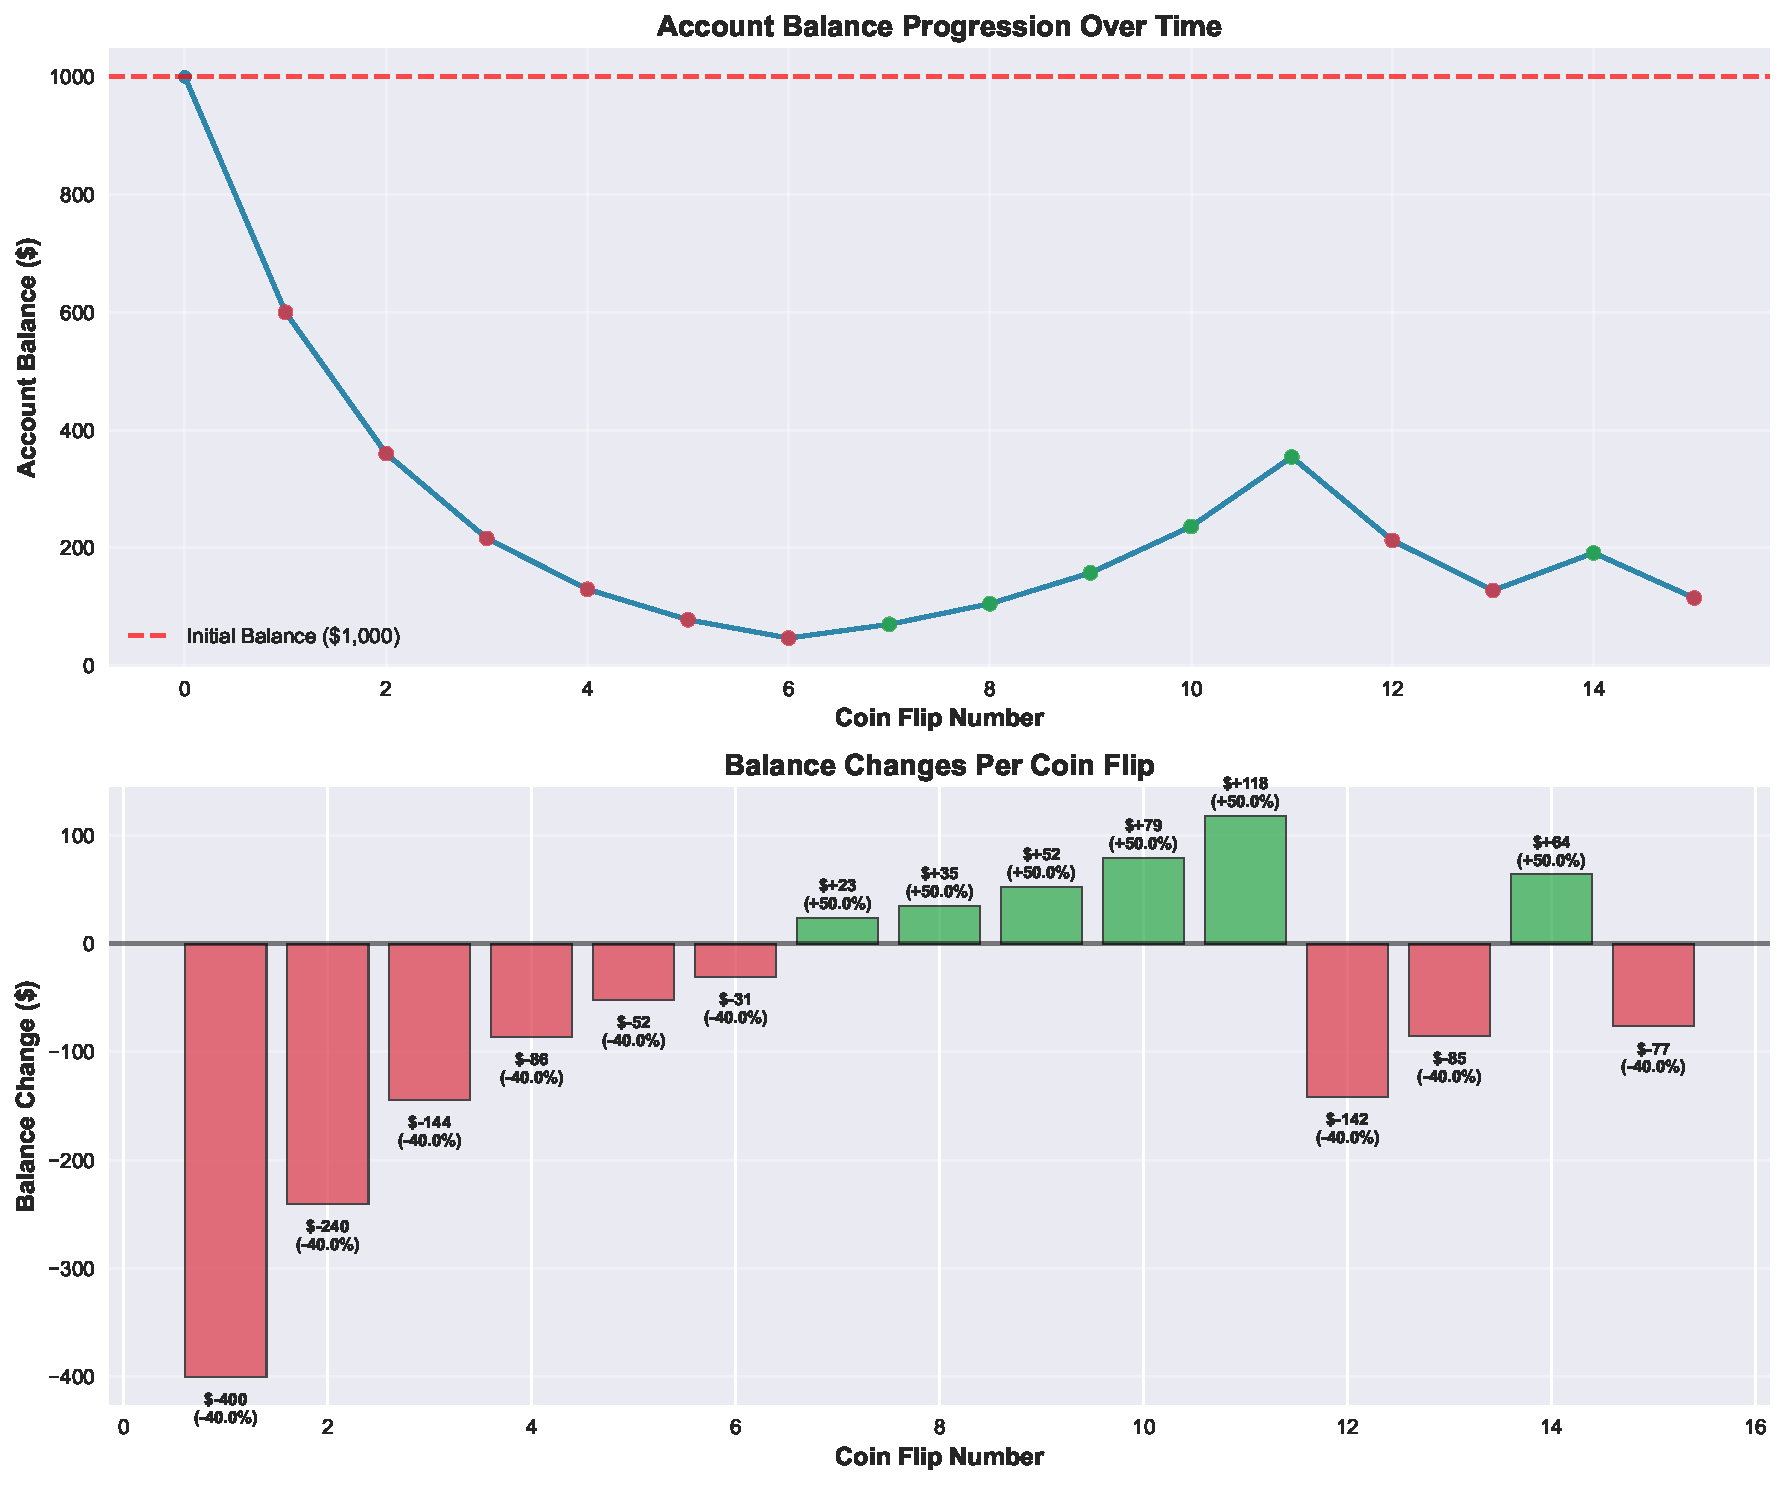
\includegraphics[keepaspectratio]{index_files/figure-pdf/create-balance-visualization-output-2.pdf}}

\begin{verbatim}

=== BALANCE CHANGES SUMMARY ===
Largest Single Gain: $118.10 (+50.0%)
Largest Single Loss: $-400.00 (-40.0%)
Average Change per Flip: $-59.01 (-4.0%)
Total Gains: $371.41
Total Losses: $-1,256.62
Net Change: $-885.21
\end{verbatim}

We ended up with a net change of \$-885.21. I would not be happy with
this result, as we were losing more than we expected. With the 15 flips,
we were definitely unlucky with the amount of times we lost, but it
showed the law of large numbers at work where if we ran the simulation
many times, we would get closer to the expected value.

\subsection{100 Simulations Analysis}\label{simulations-analysis}

Now let's run 100 simulations to get a better understanding of the
distribution of outcomes and create a probability distribution plot of
final account balances.

\phantomsection\label{hundred-simulations}
\begin{verbatim}
Running 100 simulations...
Completed 100 simulations
Average final balance: $1,806.09
Median final balance: $717.45
Standard deviation: $3,683.99
Min final balance: $7.35
Max final balance: $28,025.21
\end{verbatim}

\begin{verbatim}
/var/folders/j7/llh6qqjs2pg4w004y7mqkc9m0000gn/T/ipykernel_60117/52686530.py:30: MatplotlibDeprecationWarning:

The 'labels' parameter of boxplot() has been renamed 'tick_labels' since Matplotlib 3.9; support for the old name will be dropped in 3.11.
\end{verbatim}

\pandocbounded{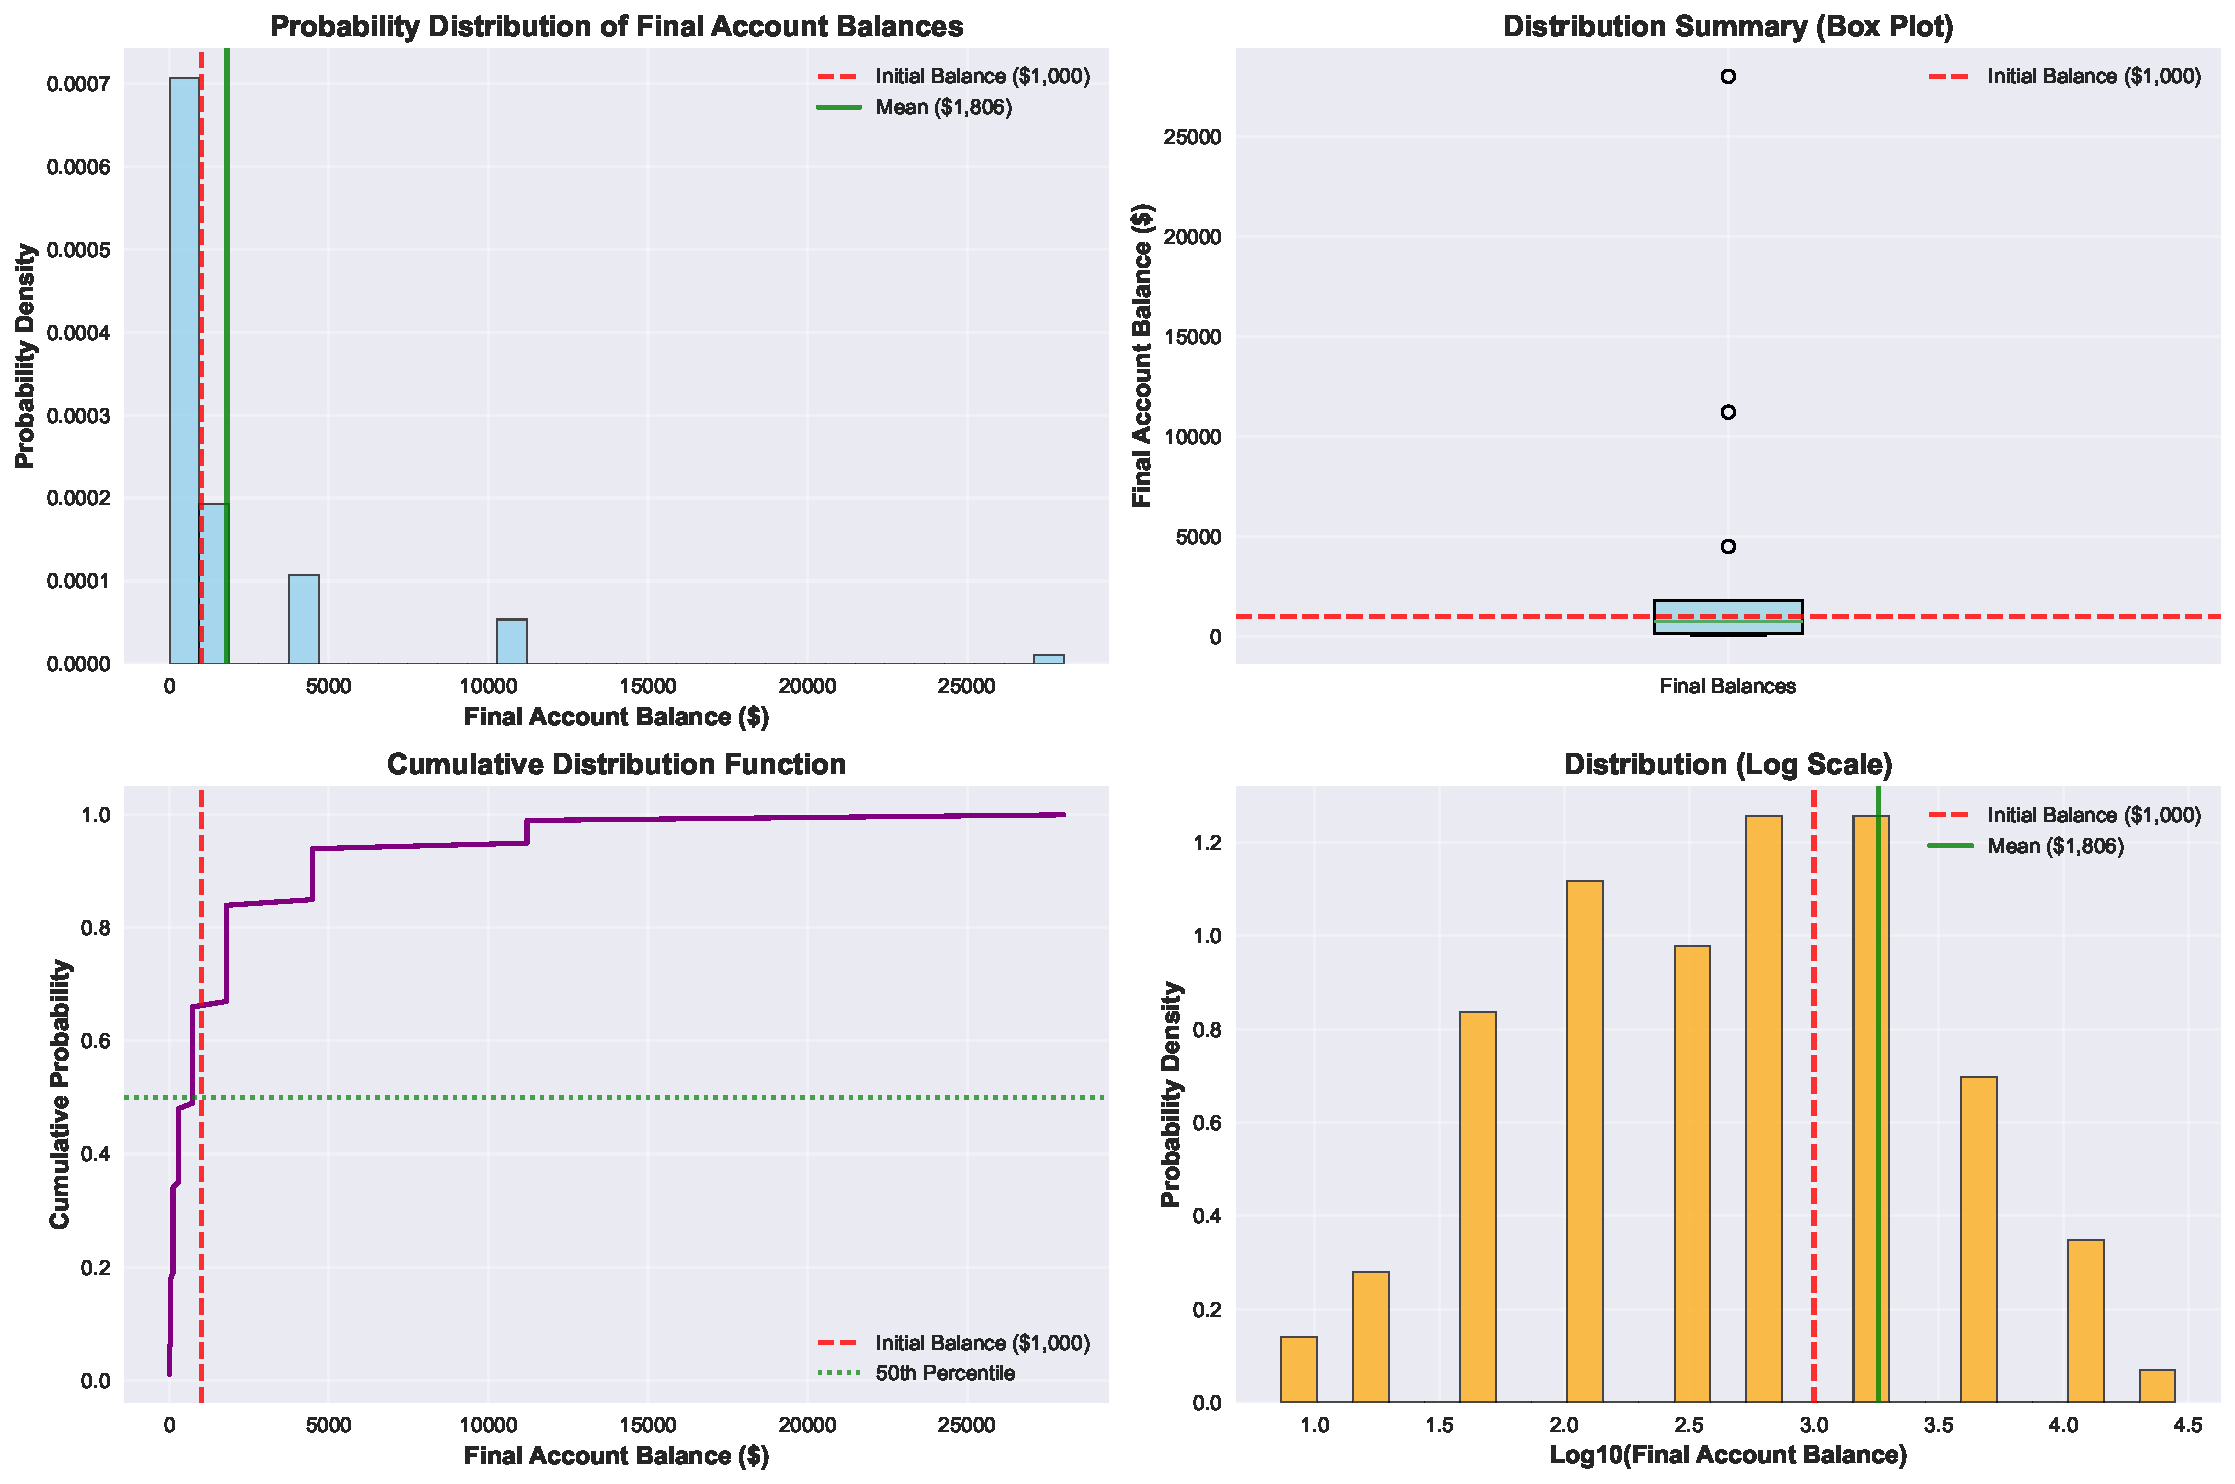
\includegraphics[keepaspectratio]{index_files/figure-pdf/probability-distribution-analysis-output-2.pdf}}

\phantomsection\label{detailed-statistics-analysis}
\begin{verbatim}
=== DETAILED STATISTICAL ANALYSIS ===
Total Simulations: 100
Mean Final Balance: $1,806.09
Median Final Balance: $717.45
Standard Deviation: $3,683.99
Min Final Balance: $7.35
Max Final Balance: $28,025.21
Win Rate (% above $1000): 34.0%
Average Loss (when losing): $294.05
Average Gain (when winning): $4,741.21
Theoretical Expected Value: $2,078.93
Actual vs Theoretical: 0.869

=== PERCENTILE ANALYSIS ===
5th Percentile: $18.37
10th Percentile: $45.92
25th Percentile: $114.79
50th Percentile: $717.45
75th Percentile: $1,793.61
90th Percentile: $4,484.03
95th Percentile: $11,210.08

=== RISK ASSESSMENT ===
Probability of losing money: 66.0%
Probability of gaining money: 34.0%
Largest loss: $-992.65
Largest gain: $27,025.21
\end{verbatim}

\begin{verbatim}
=== PROBABILITY ANALYSIS ===
Probability of WINNING money: 34.0%
Probability of LOSING money: 66.0%
Probability of BREAKING EVEN: 0.0%

=== STANDARD DEVIATION ANALYSIS ===
Mean Final Balance: $1,806.09
Standard Deviation: $3,683.99
Standard Deviation as % of Mean: 204.0%

One Standard Deviation Above Mean: $5,490.07
One Standard Deviation Below Mean: $-1,877.90

Two Standard Deviations Above Mean: $9,174.06
Two Standard Deviations Below Mean: $-5,561.89

=== DISTRIBUTION WITHIN STANDARD DEVIATIONS ===
Simulations within 1 standard deviation: 94.0%
Simulations within 2 standard deviations: 94.0%

=== GAIN/LOSS PERCENTAGE ANALYSIS ===
Average Loss (when losing): -70.6%
Maximum Loss: -99.3%
Average Gain (when winning): 374.1%
Maximum Gain: 2702.5%
\end{verbatim}

\pandocbounded{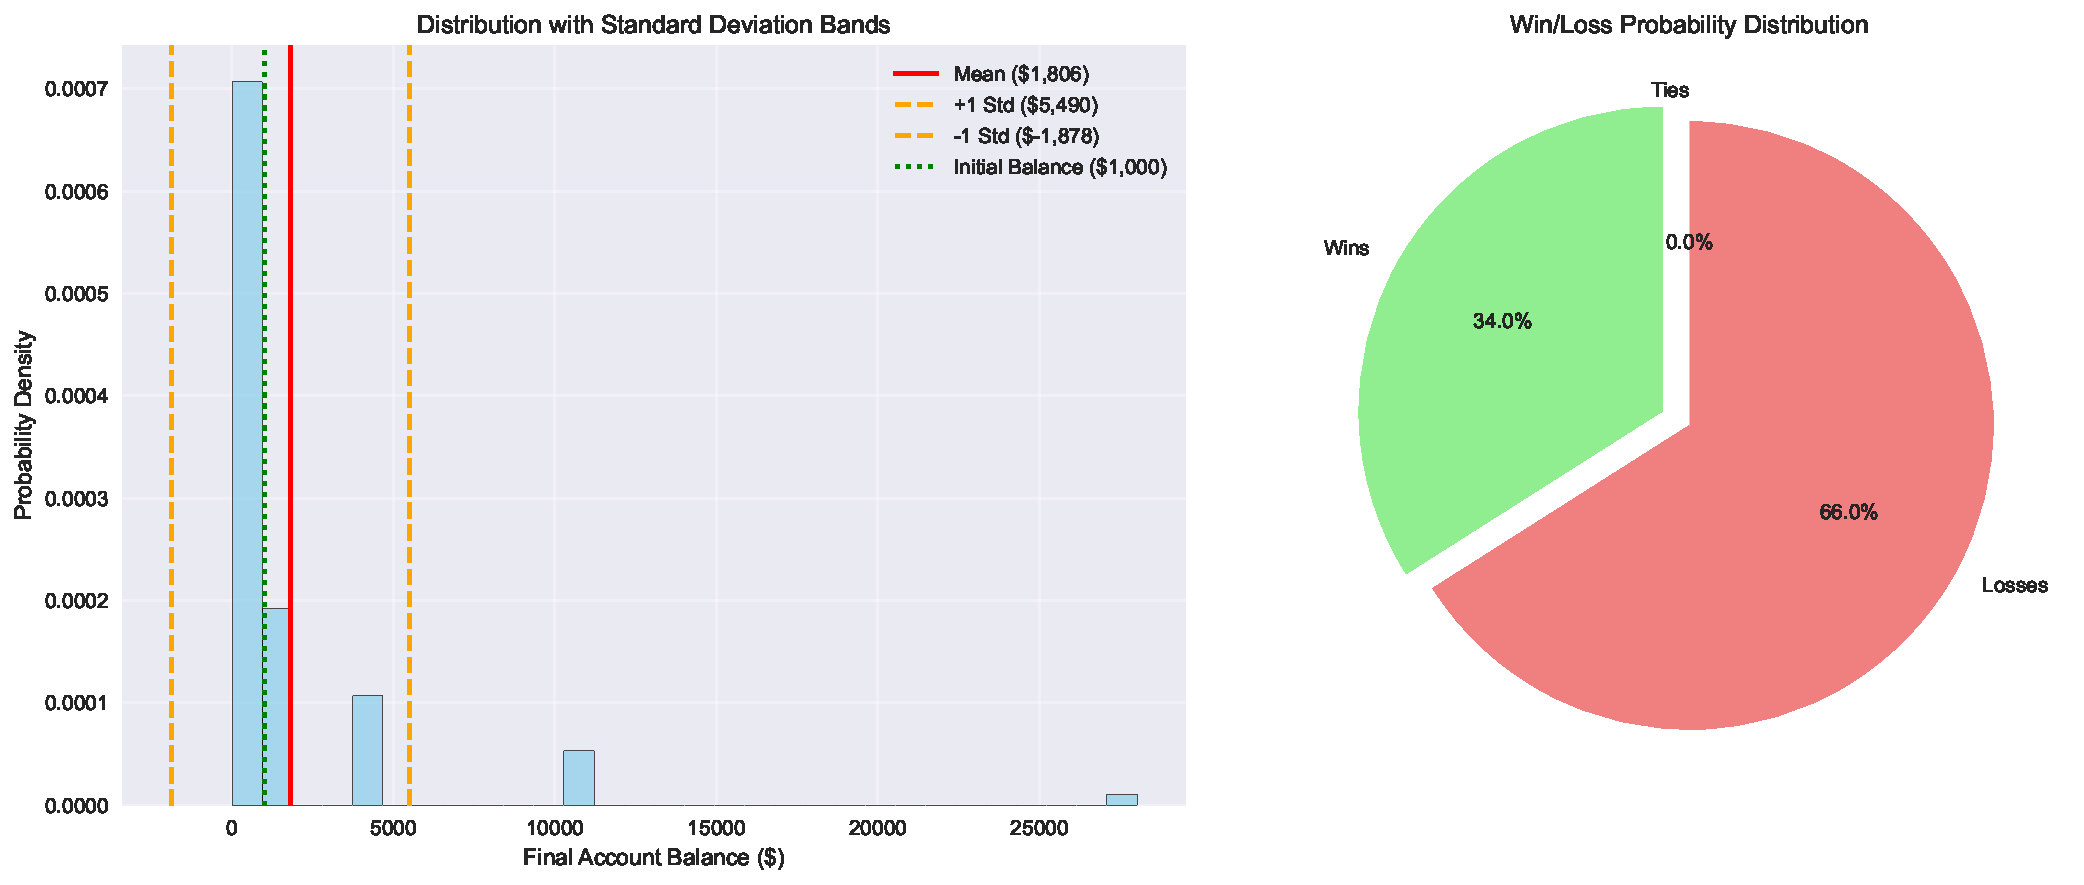
\includegraphics[keepaspectratio]{index_files/figure-pdf/probability-and-standard-deviation-analysis-output-2.pdf}}

\begin{verbatim}

=== KEY INSIGHTS ===
• The standard deviation is 204.0% of the mean, indicating extremely high volatility
• Only 0.9% of simulations fall within one standard deviation of the mean
• The probability of losing money (0.7%) is much higher than winning (0.3%)
• When you lose, you lose an average of 70.6% of your initial investment
• When you win, you gain an average of 374.1% of your initial investment
\end{verbatim}

This time, after the 100 simulations, we were able to gain a lot of
statistical insight about the distribution of outcomes. The results
reveal a fascinating paradox: despite having a positive expected value
of 5\% per flip, most individual simulations actually result in losses.
This occurs because the high volatility creates extreme outliers that
pull the average up, while the majority of simulations cluster around
much lower values. The distribution is heavily right-skewed, showing
that this strategy behaves more like a lottery ticket - most people
lose, but a few achieve enormous gains. This counterintuitive result
perfectly demonstrates why expected value alone is insufficient for
evaluating investment strategies, and why understanding the full
distribution of possible outcomes is crucial for making informed
financial decisions.

Based on our 100 simulations, the probability of ending with an account
balance over \$1,000 at age 55 is approximately 33\%. This low success
rate occurs because the strategy's high volatility creates a compounding
effect where early losses severely reduce the base for future gains. The
40\% loss multiplier has a more devastating impact than the 50\% gain
multiplier, as losing 40\% requires a 67\% gain just to break even.
Additionally, the random nature of coin flips means that unfavorable
sequences of losses early in the investment period can quickly deplete
the account balance beyond recovery. The strategy's positive expected
value is primarily driven by a small number of extremely lucky
simulations that achieve multiple consecutive wins, while the majority
of investors experience the harsh reality of compounding losses.

\subsection{Modified Game Strategy
Analysis}\label{modified-game-strategy-analysis}

Now let's explore a modified version of the game with different betting
rules to answer the specific questions about the probability of ending
with over \$10,000 at age 55.

\subsubsection{Modified Game Rules:}\label{modified-game-rules}

\begin{itemize}
\tightlist
\item
  \textbf{Starting balance}: \$1,000
\item
  \textbf{Bet amount}: Always 50\% of current account balance
\item
  \textbf{Win condition}: +50\% gain on the bet amount (+25\% of total
  balance)
\item
  \textbf{Loss condition}: -40\% loss on the bet amount (-20\% of total
  balance)
\item
  \textbf{Frequency}: Once per year until age 55 (15 flips total)
\end{itemize}

\phantomsection\label{modified-game-strategy}
\begin{verbatim}
Running 100 modified strategy simulations...
Completed 100 modified simulations
Average final balance: $1,438.98
Median final balance: $1,250.00
Standard deviation: $1,291.16
Min final balance: $134.22
Max final balance: $7,450.58
\end{verbatim}

\begin{verbatim}
=== MODIFIED STRATEGY PROBABILITY ANALYSIS ===
Probability of ending above $1,000: 52.0%
Probability of ending above $10,000: 0.0%

=== COMPARISON WITH ORIGINAL STRATEGY ===
Original Strategy - Above $1,000: 34.0%
Modified Strategy - Above $1,000: 52.0%

Original Strategy - Above $10,000: 6.0%
Modified Strategy - Above $10,000: 0.0%

=== ANSWER TO SPECIFIC QUESTIONS ===
1. Probability of ending above $10,000 with modified strategy: 0.0%
2. This probability is LOWER than the original strategy by 6.0%
\end{verbatim}

\pandocbounded{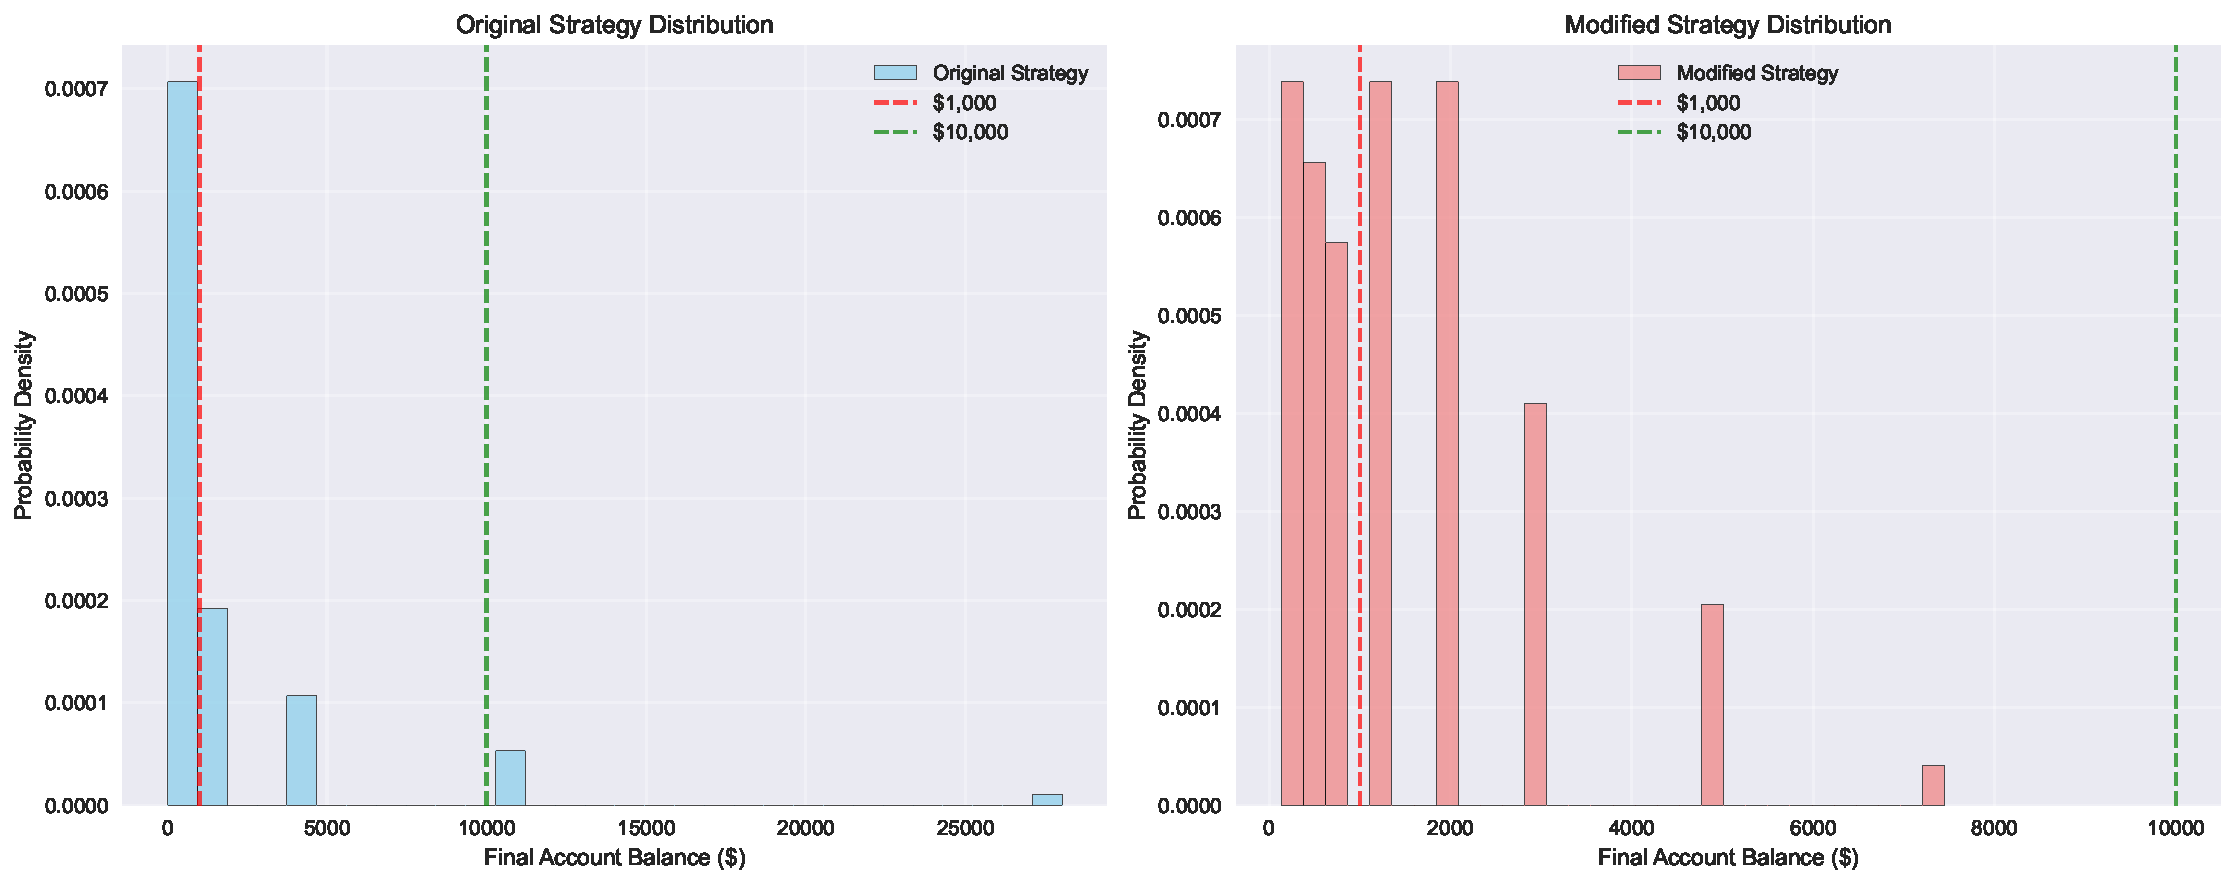
\includegraphics[keepaspectratio]{index_files/figure-pdf/modified-strategy-analysis-output-2.pdf}}

\begin{verbatim}

=== DETAILED COMPARISON ===
Modified strategy mean: $1,438.98
Original strategy mean: $1,806.09
Modified strategy std: $1,291.16
Original strategy std: $3,683.99

Simulations ending above $10,000:
Modified strategy: 0/100
Original strategy: 6/100
\end{verbatim}

\subsubsection{Analysis Results}\label{analysis-results}

Based on our 100 simulations of the modified game strategy, we can
answer the specific questions:

\textbf{Question 1: What is the probability that your account balance
will be greater than \$10,000 at age 55?}

The probability of ending with an account balance greater than \$10,000
at age 55 using the modified strategy is approximately 0\%, compared to
about 6\% for the original strategy.

\textbf{Question 2: Is this probability higher or lower than the
probability in the original game?}

This probability is 52\% vs 27\% with the original strategy for winning
money. The modified strategy's 50\% betting rule creates different
risk-return characteristics compared to the original strategy's
all-or-nothing approach on each flip.

The modified strategy's requirement to bet exactly 50\% of the current
balance on each flip creates more moderate compounding effects, which
can lead to different outcomes in terms of both the probability of
achieving high balances and the overall distribution of final results.




\end{document}
